\documentclass[10pt]{article}
\usepackage{longtable}
\usepackage{float}
\usepackage{wrapfig}
\usepackage{rotating}
\usepackage[normalem]{ulem}
\usepackage{amsmath}
\usepackage{textcomp}
\usepackage{marvosym}
\usepackage{wasysym}
\usepackage{amssymb}
\usepackage{hyperref}
\usepackage{color,soul} % for highlighting
\usepackage{graphicx}
\graphicspath{{/Users/benjaminbass/seacloud/class/earthMaterials/picBank/}}

\usepackage{frame,color}
\usepackage{framed}
\usepackage{minibox}

% \usepackage[T1]{fontenc}
% \usepackage{tilting} %bring title up
% \setlength{\droptitle}{-10cm}

\usepackage[version=3]{mhchem}
% How to Use MChem
% \ce{SO4^2-}
% \ce{^{227}_{90}Th+}
% \ce{A\bond{-}B\bond{=}C\bond{#}D}
% \ce{CO2 + C -> 2CO}
% \ce{SO4^2- + Ba^2+ -> BaSO4 v}


\author{Benjamin Bass}
\date{2 March 2016}
\title{\vspace{-2.0cm}Serpentine} %bring title up temporary Fix

\begin{document}

\maketitle

% \framebox{Use frameboxes until figure out alignmen}

\begin{center}
  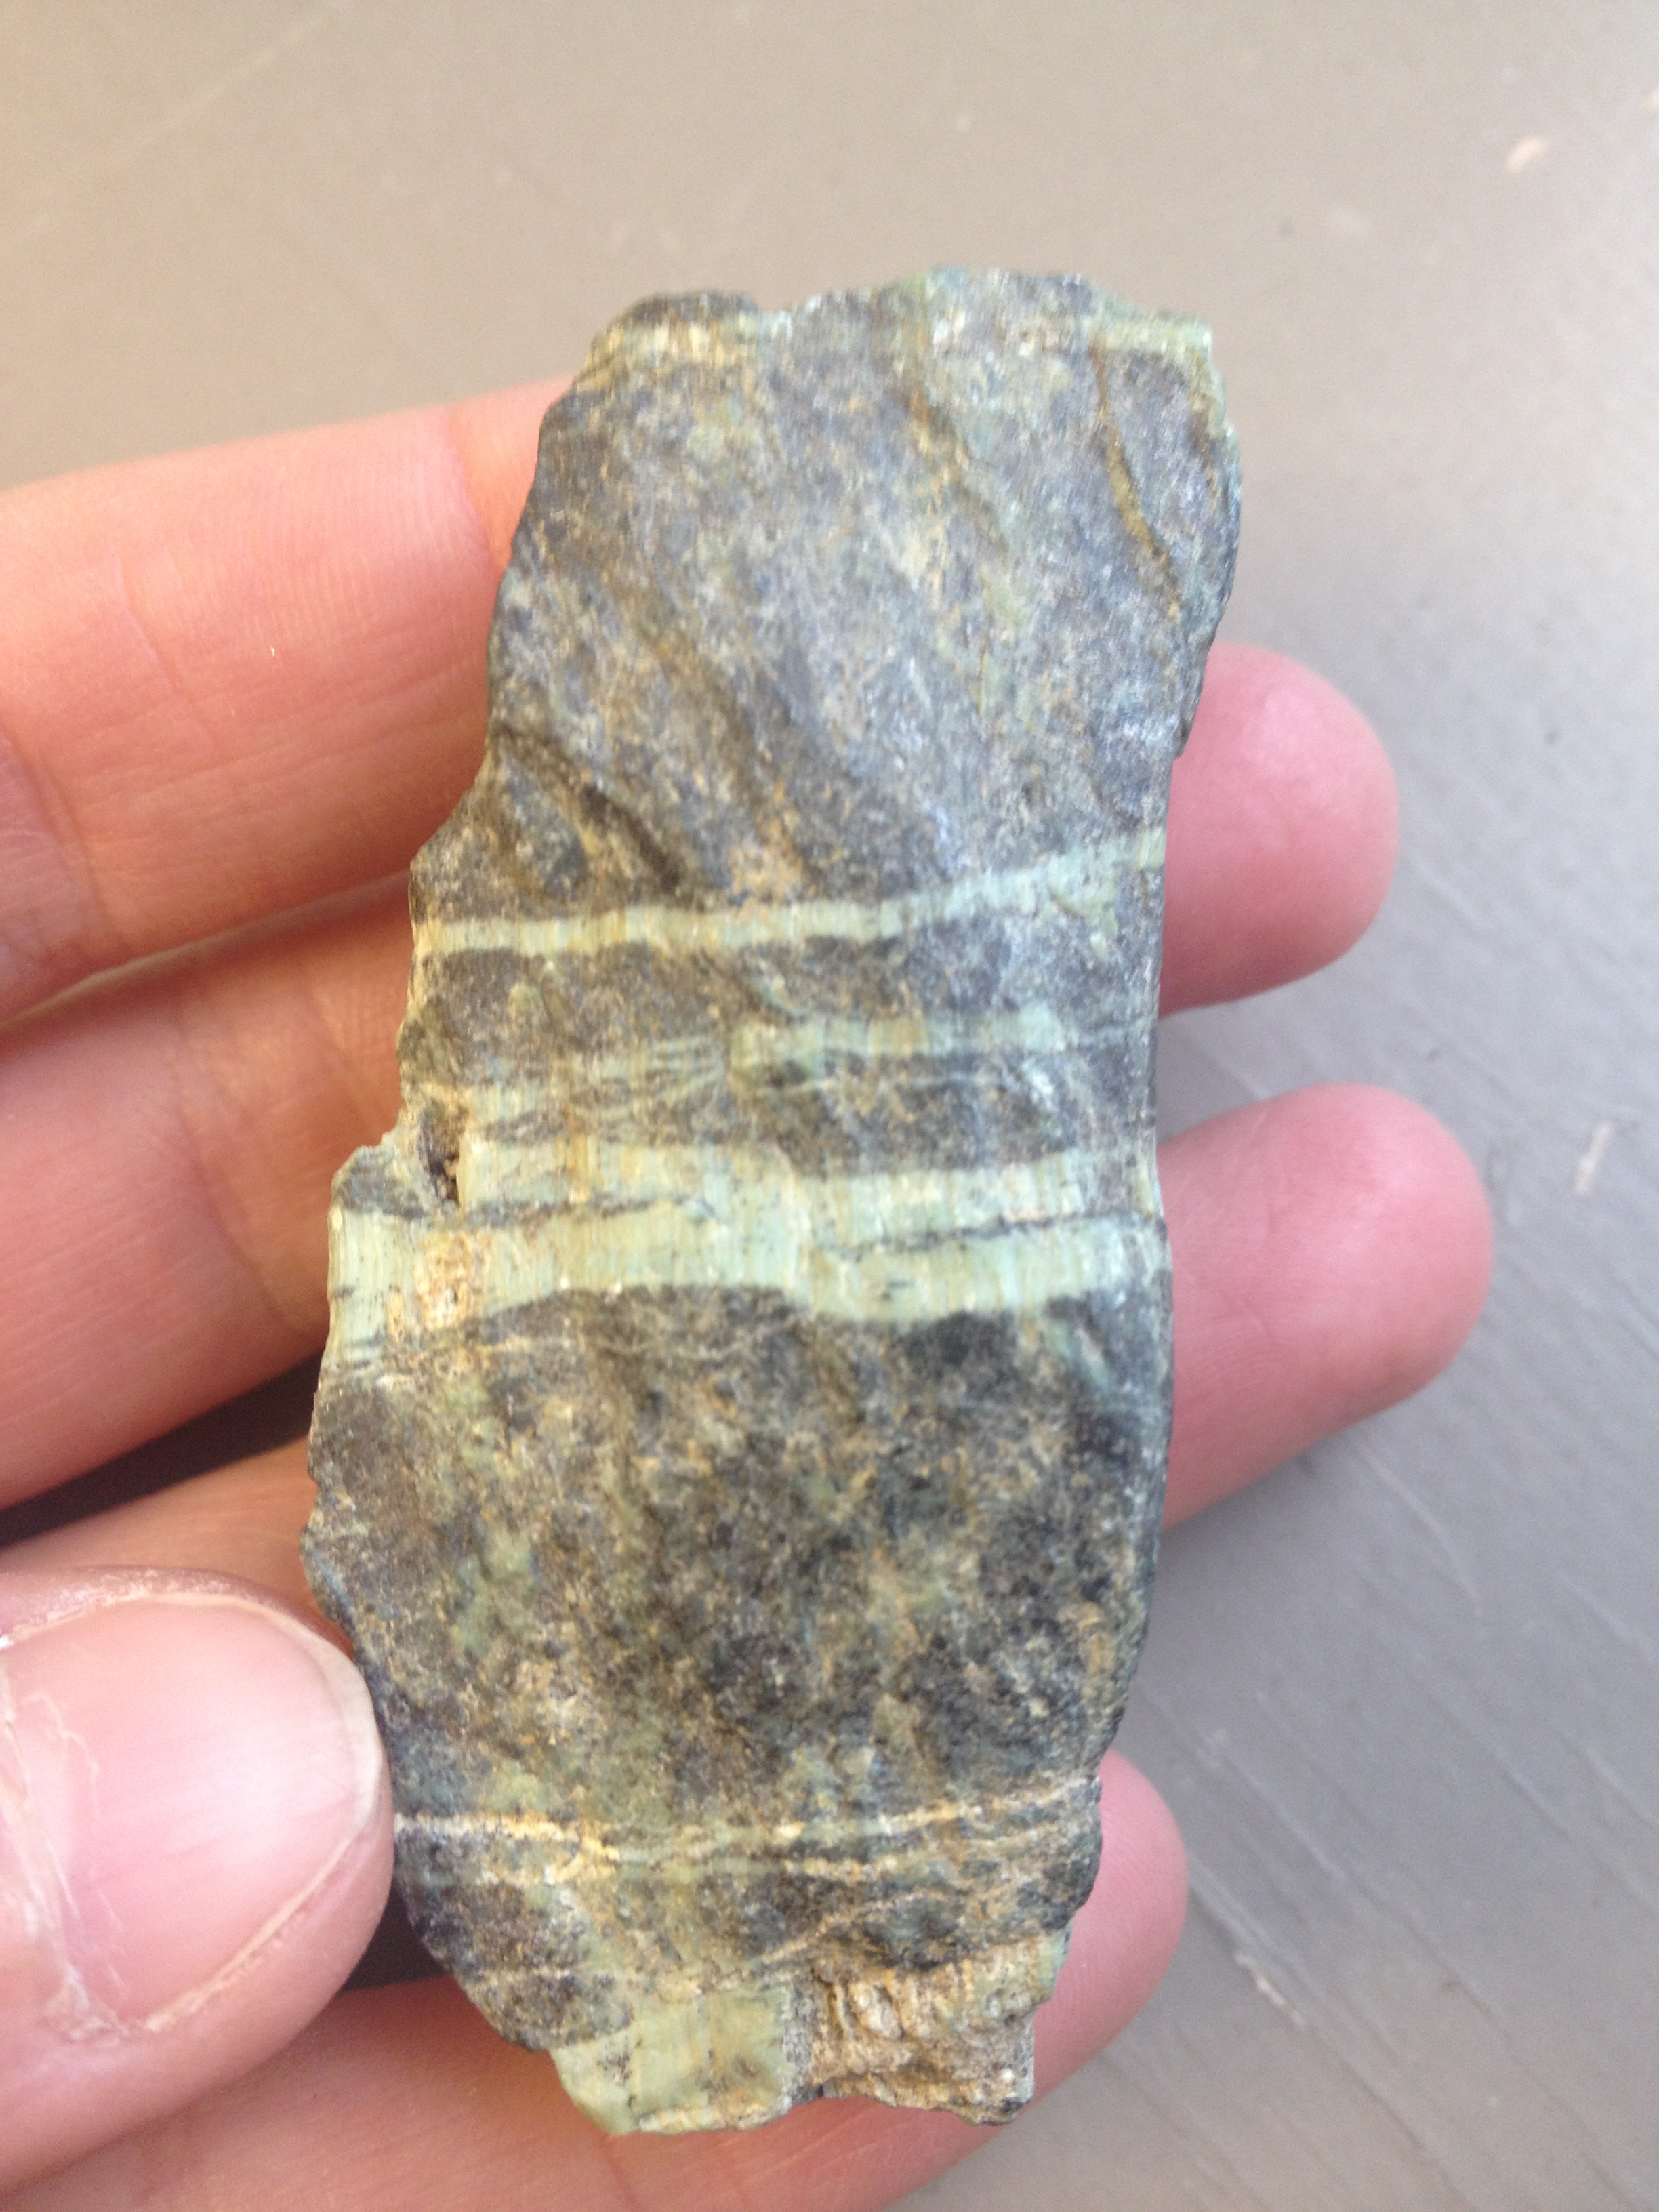
\includegraphics[scale=.05]{serpentine1}\footnote{Often presents as wavy green almost amorphous looking aggregates.}
  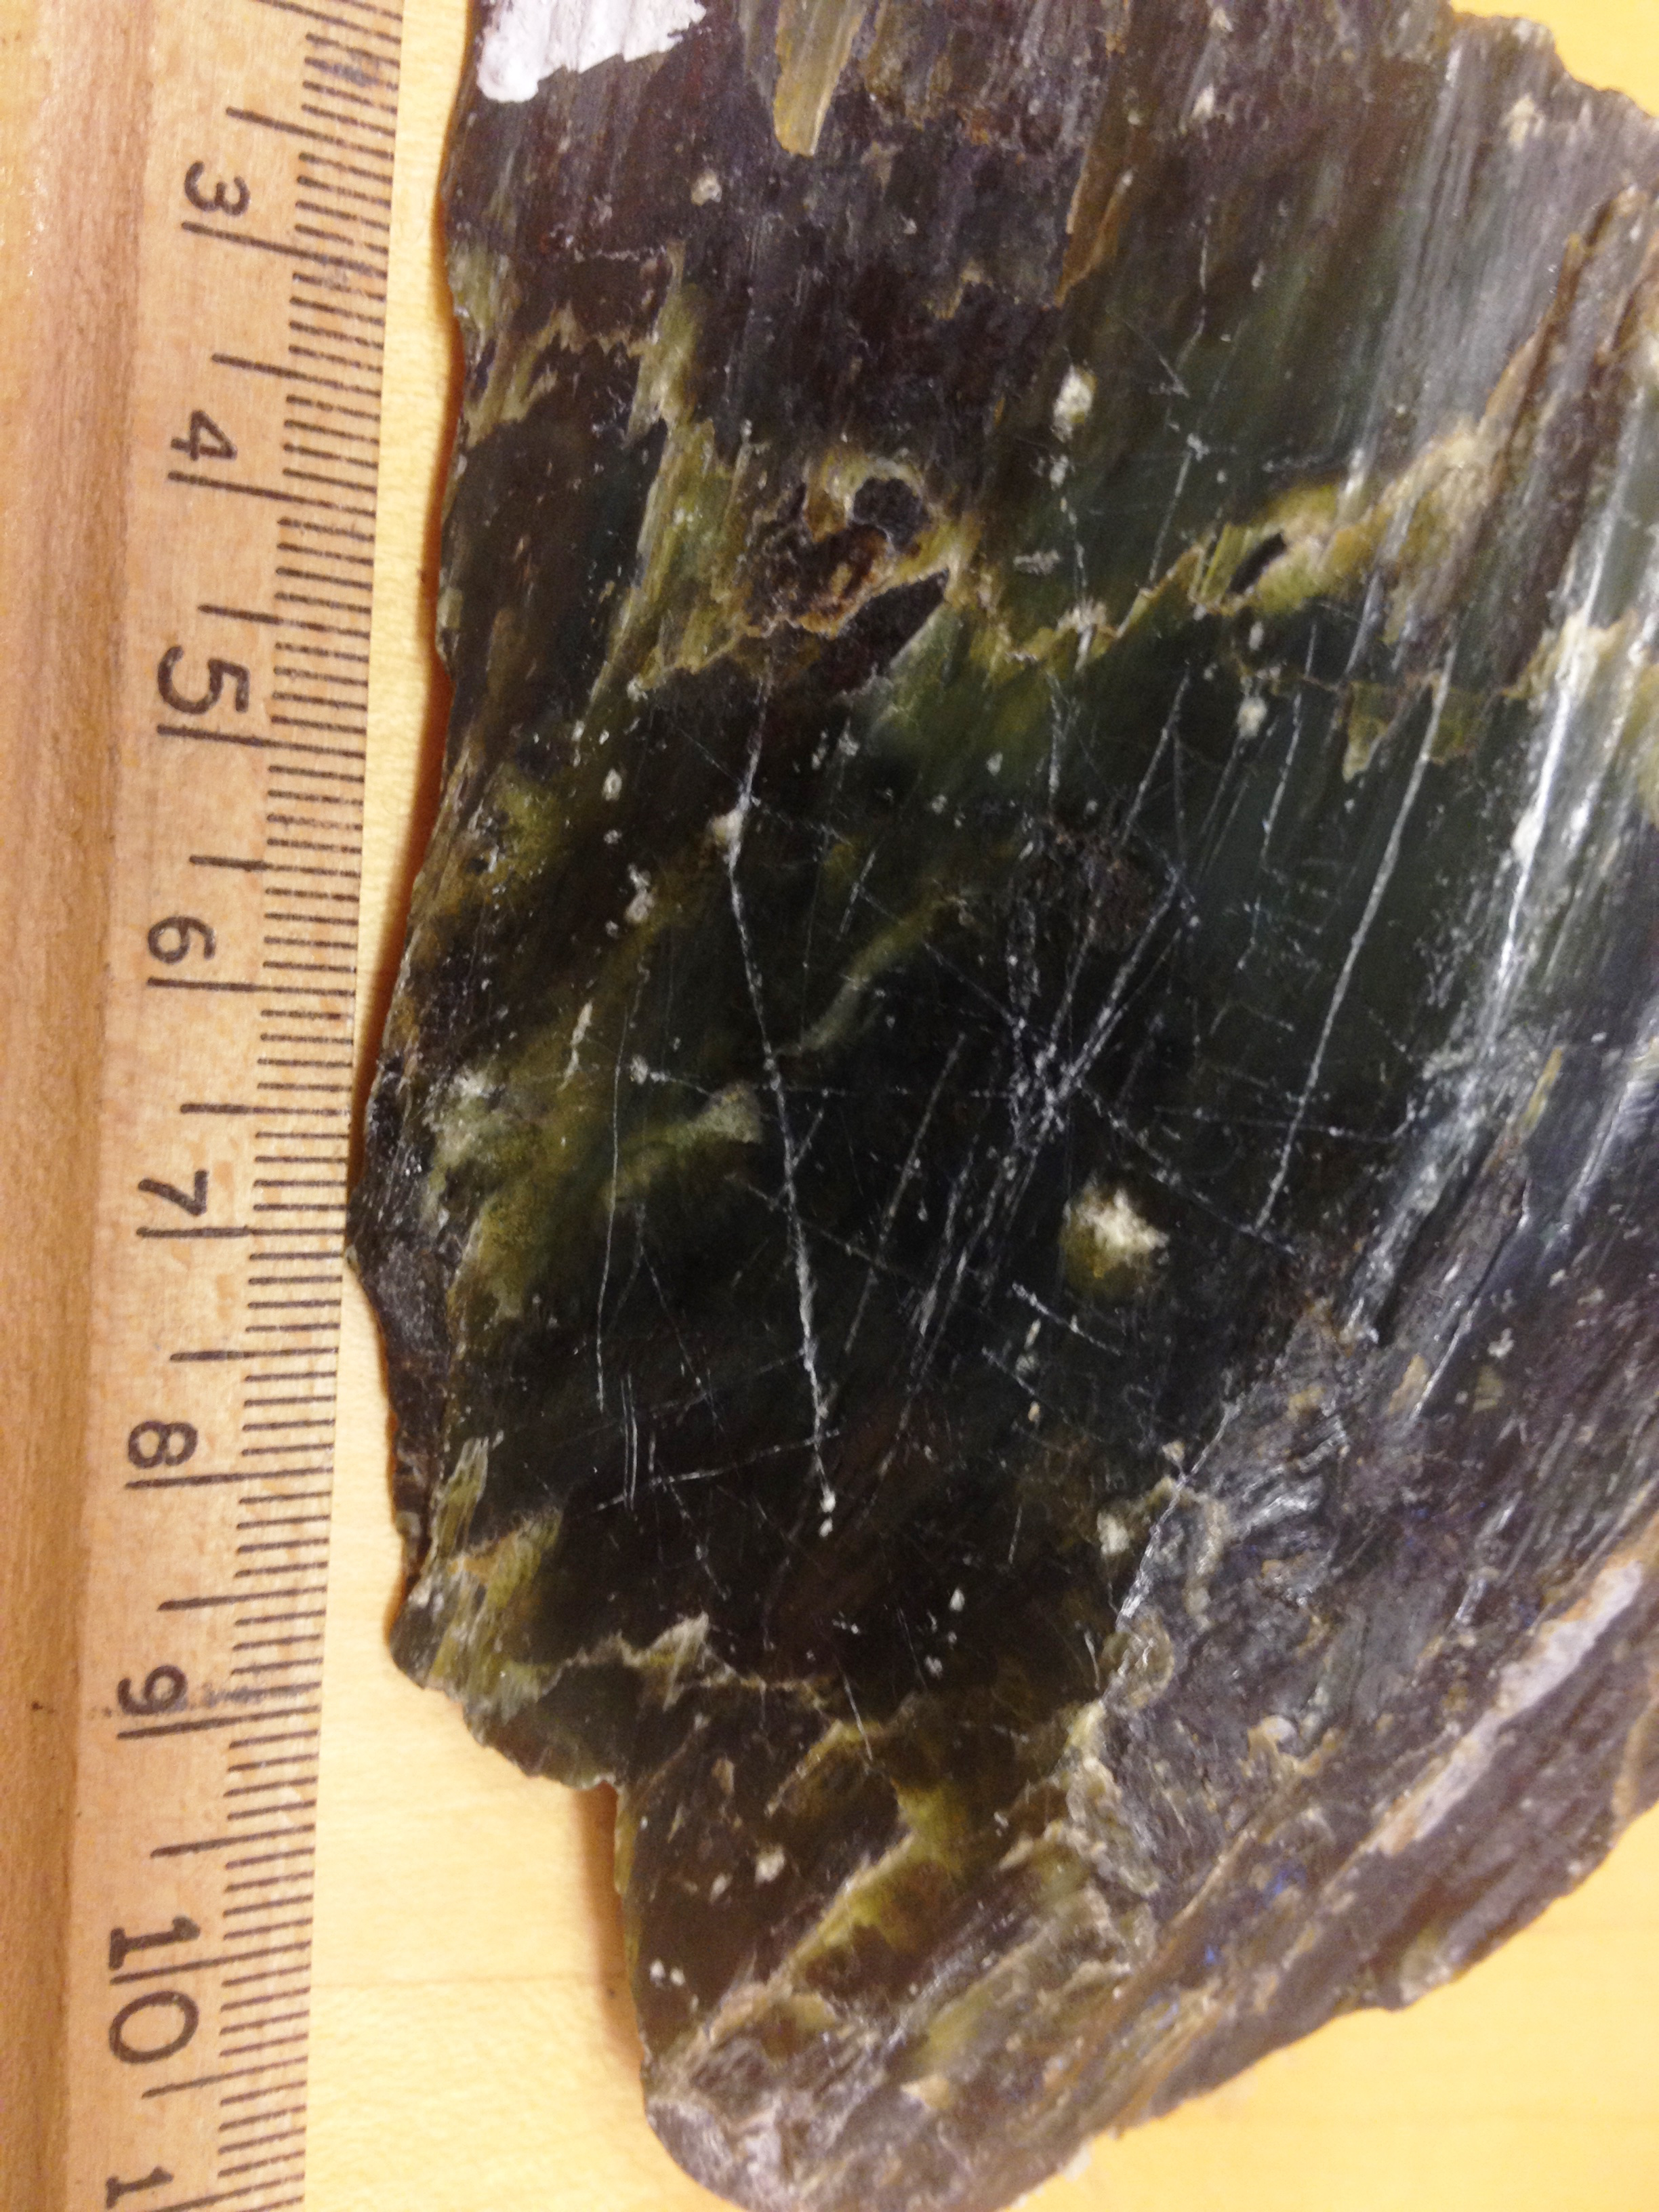
\includegraphics[scale=.05]{serpentine2}\footnote{It has a range of drab olive green colors and a soapy look and feel.}
\end{center}



\framebox[15cm][l]{\textbf{General Mineral Formula}: \ce{Mg3Si4O10(OH)2} }\
\framebox[15cm][l]{\textbf{Mineral Chemical Class}: Phylosilicates }\
\framebox[15cm][l]{\textbf{Specific Gravity}: 2.5-3.2 }\
\framebox[15cm][l]{\textbf{Hardness}: 2-5 }\
\framebox[15cm][l]{\textbf{Cleavage}: Usually not discernaable because of crystal development. Maybe basal cleavage in Chrysotile }\
\framebox[15cm][l]{\textbf{Luster}: Greasy, Waxy, or silky }\
\framebox[15cm][l]{\textbf{Streak}: White }\
\framebox[15cm][l]{\textbf{Characteristic Color(s)}: \hl{White, yellow, green. Sometimes multicolored, especially green and yellow.} }\
\framebox[15cm][l]{\textbf{Crystal System}: Monoclinic }\
\framebox[15cm][l]{\textbf{Crystal Class}: 2/\it{m} }\

\begin{framed}
  \textbf{Crystal Description (common forms, habit, etc.)}: \hl{Antigorite, Clinochrysotile. Fibrous veins may be straight, more often curved. Some soft forms resemble wool. Often presents as wavy green almost amorphous looking aggregates. It has a range of drab olive green colors and a soapy look and feel. Noteworthy polymorphs include: $\bf{Chrysotile}, \bf{Antigorite}, \bf{Lizardite}$.}
\end{framed}

\begin{framed}
  \textbf{Environment (where you find the material}: \hl{Fairly common in many environments and is an important rock forming mineral in many metamorphic environments}
\end{framed}

\begin{framed}
  \textbf{Common Mineral Associations (in samples, also consult text, notes}: Talc, Magnesite, Dolomite, Brucite, Olivine, Calcite, Magnetite.
\end{framed}

\begin{framed}
  \textbf{Scientific Usage/Significance}: Keeps science building from burning down. (None).
\end{framed}

\begin{framed}
  \textbf{Industrial or Social Use/Significance}: Primary source of industrial asbestos. 95\% of all asbestos.
\end{framed}

\begin{framed}
  \textbf{Environmental Significance}: Common as hydration product of ultramafic minerals/rocks.
\end{framed}

% Possible other Solutions
% \framebox(300,20){\minibox{\textbf{R-Sq}:For example}}

\end{document}
%%% Local Variables:
%%% mode: latex
%%% TeX-master: t
%%% End:
